\documentclass[ex]{exercise}

\deadline{24.10.2023}

\begin{document}

\section{Listingsche Strahlenkonstruktion an Hohl- und Wölbspiegel}
\hfill(siehe hinten)\hspace*{\fill}
\vspace{-0.3cm}

\section{Spiegelprisma}
\begin{figure}[h]
    \centering
    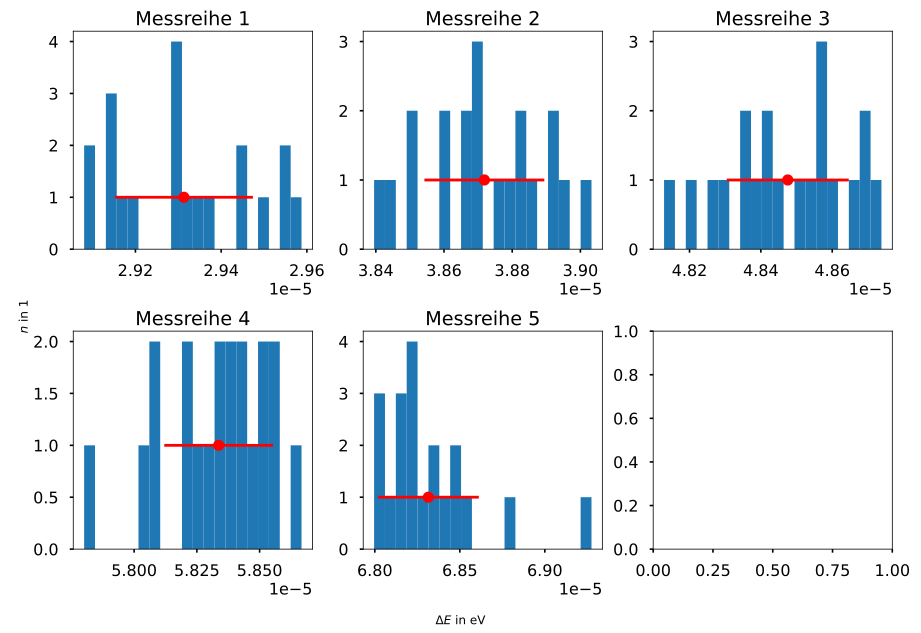
\includegraphics[width=0.8\textwidth]{1.jpg}
    \caption{Skizze der Geometrie und Rechnung}
\end{figure}
\vspace{-0.5cm}
\begin{align*}
    \tilde \beta &= \arcsin\hug{\frac{n_b}{n_a} \sin\hug{\frac{\pi}{3}-\arcsin\hug{\frac{n_a}{n_b} \sin \alpha}}}\\
    &\approx \arcsin\hug{\frac32 \sin\hug{\frac{\pi}{3}-\arcsin\hug{\frac23 \sin \frac{\pi}{3}}}}\\
    &\approx 0.679 \approx 38.9^\circ
\end{align*}

\section{Glasfaserkabel}
\begin{align*}
    \frac{\sin\alpha}{\sin\beta} &= \frac{n_b}{n_a}\\
    \frac{\sin\alpha_{0}}{\sin\frac\pi2} &= \frac{n_b}{n_a}
\end{align*}\vspace{-0.6cm}
\begin{align*}
    \alpha_{0} = \arcsin\frac{n_b}{n_a}
    \approx \arcsin\frac{1.52}{1.66}
    \approx 1.16 \approx 66.3^\circ 
\end{align*}
Totale interne Reflexion tritt für Winkel \(\alpha\le\alpha_0\) auf.\\

\begin{figure}[H]
    \centering
    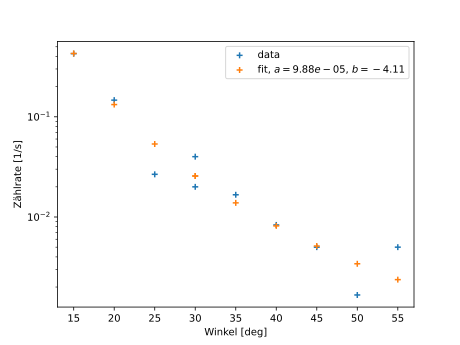
\includegraphics[width=0.4\textwidth]{2.jpg}
    \caption{Skizze eines gekrümmten Kabels}
\end{figure}

Wie aus der Skizze erkenntlich wird gilt:
\begin{align*}
    \sin\alpha_0 &= \frac{r_{min}-r_i}{r_{min}}\\
    \\
    r_{min} &= \frac{r_i}{1-\sin\alpha_0} = \frac{r_i}{1-\frac{n_b}{n_a}}\\
    &\approx \frac{1\u{mm}}{1- \frac{1.52}{1.66}}
    \approx 11.9 \u{mm} 
\end{align*}

\section{Katakaustik}
\begin{align*}
    y_\varphi(x) %&= R\cdot \cos\varphi- \tan(2\varphi)(x-R\cdot \sin(\varphi))\\
    &= R\cdot (\cos\varphi + \sin(\varphi)\tan(2\varphi)) - \tan(2\varphi)x\\
    \\
    0 &= \partiald{y_\varphi}{\varphi} \\
    &= R\frac{3\sin\varphi + \sin(3\varphi)}{2\cos^2(2\varphi)} - \frac{2}{\cos^2(2\varphi)}x\\
    x &= \frac R4\hug{3\sin\varphi + \sin(3\varphi)}\\
    \\
    \vec x(\varphi) &= R \twovec{\frac 14\hug{3\sin\varphi + \sin(3\varphi)}}
    {\cos\varphi + \sin(\varphi)\tan(2\varphi) - \frac 14\tan(2\varphi)\hug{3\sin\varphi + \sin(3\varphi)}}\\
    &= \frac R4 \twovec{3\sin\varphi + \sin(3\varphi)}
    {4\cos\varphi + \tan(2\varphi)\hug{\sin\varphi - \sin(3\varphi)}}\\
    &= \frac R4 \twovec{3\sin\varphi + \sin(3\varphi)}
    {3\cos\varphi + \cos(3\varphi)}
\end{align*}

\includepdf[pages=1-2]{blatt2.pdf}
\end{document}